\documentclass[11pt,a4paper,sans]{moderncv}
\moderncvstyle{banking}
\moderncvcolor{blue}

\usepackage[scale=0.75]{geometry}
\usepackage[utf8]{inputenc}
\usepackage[T1]{fontenc}
\usepackage{graphicx}
\usepackage{enumitem}


\begin{document}

\beforetitle{
  \vspace*{-2em}
  \begin{center}
    {\Huge\sffamily\bfseries French-speaking} \\[0.3em]
    {\Huge\sffamily Agile Project Manager} \\[0.4em]
    {\color{gray}\large\sffamily Fullstack Developer – GTFS, OSM, PostGIS} \\[1em]
    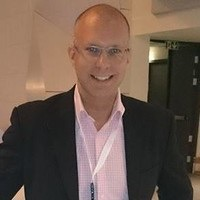
\includegraphics[width=3.6cm]{./photos/rickardaberg-consultant.jpeg} \\[1em]
    {\Large\sffamily Rickard \textbf{\AA{}berg}} \\[-0.3em]
    {\normalsize\sffamily MSc in Software Engineering} \\[0.5em]
    {\small\sffamily 
      \textbf{Tel:} +46 709 43 14 01 \quad 
      \textbf{Email:} rickard.aaberg@icloud.com \quad 
      \textbf{Malmö, Sweden}
    }
  \end{center}
  \vspace{0.5em}
}


% % Personal data
% \name{Rickard}{\AA{}berg}
% \title{Agile Project Manager | MSc Software Engineering} 
% \address{Bodekullsgatan 34b}{21440 Malm\"o, Sweden}{}
% \phone[mobile]{+46~709~43~14~01}
% \email{rickard.aaberg@icloud.com}
% %\photo[64pt][0.4pt]{photos/rickardaberg-consultant.jpeg}  % Adjusted path to avoid leading ./
% 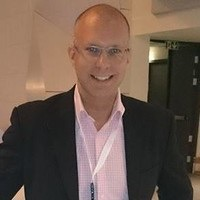
\includegraphics[width=3.6cm]{./photos/rickardaberg-consultant.jpeg} \\[1em]
% \begin{document}

% \makecvtitle

% ==== Professional Summary ====
\section{Professional Summary}
\cvitem{}{Senior Agile Project Manager and Consultant with over 10 years of experience leading cross-functional teams in international environments. Specialized in GDPR compliance, DevOps transformation, trauma-informed group facilitation, and agile delivery. Fluent in Swedish, English, and French (C1). Proven success in telecom, finance, healthcare, and public sector projects. Strong technical background in Java, DevOps toolchains, and fullstack environments. Academic foundation includes leadership, software quality, agile methods (XP), organizational behavior, and technical French, with international experience in France.}

% ==== Languages ====
\section{Languages}
\cvitemwithcomment{Swedish}{Native}{}
\cvitemwithcomment{English}{Professional proficiency}{}
\cvitemwithcomment{French}{C1 – Used professionally at \'{E}cole des Mines, Nantes. Studied technical French with immersion in La Rochelle.}{}

% ==== Certification Badges ====
\section{Certification Badges}
\cvitem{}{
  \begin{minipage}[t]{0.24\linewidth}
    \centering
    
\includegraphics[width=0.9\linewidth]{images/azure-fundamentals-badge.png}\\
    \scriptsize Microsoft Certified: Azure Fundamentals (AZ-900)
  \end{minipage}
  \hfill
  \begin{minipage}[t]{0.24\linewidth}
    \centering
    \includegraphics[width=0.6\linewidth]{images/icc_coach.jpeg}\\
    \scriptsize ICC Certified Coach
  \end{minipage}
  \hfill
  \begin{minipage}[t]{0.24\linewidth}
    \centering
    
\includegraphics[width=0.6\linewidth]{images/ISQTB.jpg}\\
    \scriptsize ISTQB Certified Tester\\Foundation Level (CTFL)
  \end{minipage}
  \hfill
  \begin{minipage}[t]{0.24\linewidth}
    \centering
    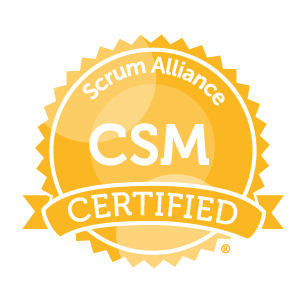
\includegraphics[width=0.9\linewidth]{images/Certified_Scrum_Master_(CSM)_certification_badge.PNG}\\
    \scriptsize Certified Scrum Master
  \end{minipage}
}

\cvitem{}{
  \begin{minipage}[t]{0.24\linewidth}
    \centering
    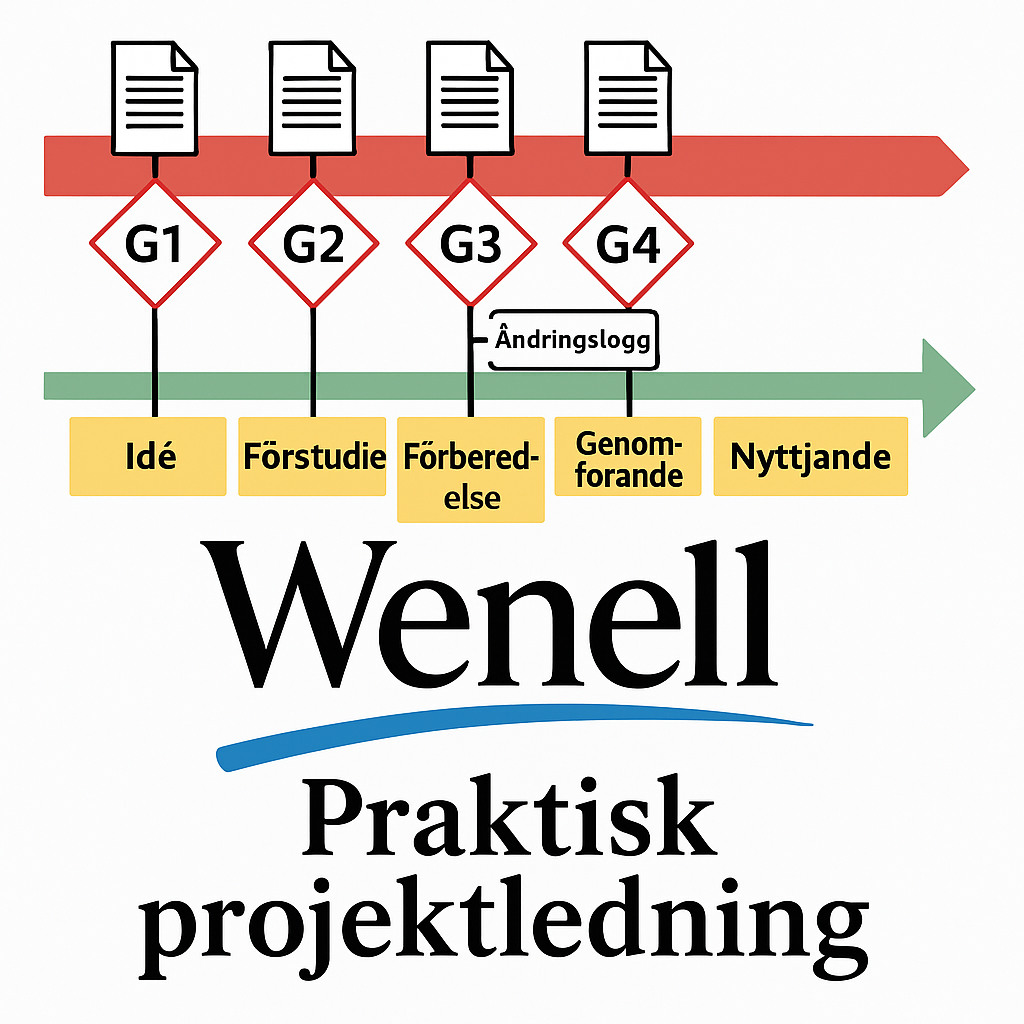
\includegraphics[width=0.9\linewidth]{images/wenell-ppl-badge.png}\\
    \scriptsize Practical Project Management (Wenell)
  \end{minipage}
  \hfill
  \begin{minipage}[t]{0.24\linewidth}
    \centering
    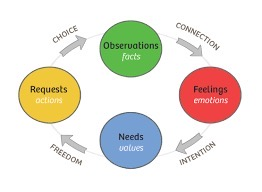
\includegraphics[width=0.9\linewidth]{images/nvc-year-badge.JPEG}\\
    \scriptsize 1-Year Program in Nonviolent Communication (NVC)
  \end{minipage}
  \hfill
  \begin{minipage}[t]{0.24\linewidth}
    \centering
    
\includegraphics[width=0.8\linewidth]{images/IMT_Atlantique_logo_1.png}\\
    \scriptsize \'{E}cole des Mines de Nantes
  \end{minipage}
  \hfill
  \begin{minipage}[t]{0.24\linewidth}
    \centering
    
\includegraphics[width=0.9\linewidth]{images/liu-logo.png}\\
    \scriptsize Link\"opings Tekniska H\"ogskola (LiTH)
  \end{minipage}
}

% ==== Key Project Experience ====
\section{Selected Projects}

\cventry{2025–}{Project Manager, VNS + HRV Tracking}{RMTS for Depression}{Malm\"o, Sweden}{}{
Led a project using Vagus Nerve Stimulation and HRV tracking to support patients with anxiety, stress, and depression. Integrated signal processing tools (DFT, FFT) and Arduino-based hardware. Agile leadership using Kanban and Trello.
}

\cventry{2020–2025}{Trauma-Informed Facilitator (Volunteer)}{ACOA via Zoom}{Remote}{}{
Facilitated over 100 trauma-sensitive peer-support meetings using IFS and NVC principles. Developed transferable skills in group regulation, deep listening, and Scrum-style moderation (timeboxing, group conscience).
}

\cventry{2017–2018}{Sub Project Manager, GDPR Compliance}{Verisure Innovation}{Malm\"o, Sweden}{}{
Managed internal GDPR compliance project for employee-facing apps. Coordinated legal, IT and product teams to implement consent and transparency features.
}

\cventry{2014–2015}{Senior PM / Scrum Master}{Nordea}{Copenhagen, Denmark}{}{
Drove DevOps transformation and agile coaching across infrastructure and development teams. Facilitated agile ceremonies, vendor coordination (AWS, Tibco), and hands-on contributions in Java and Spring Boot.
}

\cventry{2012–2014}{DevOps Lead / PM}{IKANO Bank}{Nordic Region}{}{
Led rollout of CI/CD practices, tools (CA Lisa/Nolio, Jenkins), and cross-country knowledge transfer. Reduced deployment errors and resourcing by 75\%. Technologies included .NET, BizTalk, SQL Server.
}

\cventry{2008–2009}{Project Coordinator, Custom Worktop}{IKEA IT}{\"Almhult, Sweden}{}{
Managed IT rollout across multiple countries for customized kitchen worktop ordering system. Bridged global systems and local operations.
}

\cventry{2002–2003}{Project Manager (Academic J2EE Project)}{Institution for Health and Medical Engineering}{Link\"oping, Sweden}{}{
Led student development of a J2EE application for diabetes patients in a medical technology collaboration project (MEDPUM).}



\section{Development Experience}
\cvitem{}{In addition to my project management and leadership work, I have consistently contributed hands-on as a developer and technical architect. My development experience includes:}
\begin{itemize}
  \item Fullstack developer roles using Java, Spring Boot, JavaScript/React, .NET, and Python.
  \item Integration specialist for BPM and middleware platforms such as TIBCO, MuleSoft, and BizTalk.
  \item Technical lead on deployment pipelines and CI/CD infrastructure (CA Lisa, Jenkins, Docker/Kubernetes).
  \item Jira plugin development using Java and Velocity.
  \item Contributed to award-winning BPM system integrations using SOAP/REST, JMS, and web services.
  \item Authored architectural documentation based on TOGAF, Kruchten 4+1, and Zachman frameworks.
  \item Research & development on AOP and J2EE at \'{E}cole des Mines and Vienna Component Framework.
\end{itemize}
% ==== Education ====
\section{Education}
\cventry{1996--2003}{MSc in Computer Science and Engineering}{Link\"opings Tekniska H\"ogskola}{}{}{Focus in Security, AI, Embedded, Real-time. Profiled in project management, software quality, agile methods (XP), leadership (Yukl), organizational behavior, IT strategy and entrepreneurship. Included coursework in technical and economic French with language exchange in La Rochelle.}
\cventry{2003--2004}{R\&D Engineer / MSc Thesis}{\'{E}cole des Mines de Nantes}{France}{}{Internship and thesis on component frameworks and AOP. Employed post-thesis as Java developer and researcher in J2EE and Linux kernel evolution.}

% ==== Technical Skills Summary ====
\section{Technology Stack Summary}
\cvitem{Languages}{Java, Python, JavaScript (React), SQL, Lisp, OCaml, C, Assembler}
\cvitem{Frontend}{React, Angular, Vue, HTML/CSS, Bootstrap}
\cvitem{DevOps}{Jenkins, Git, Docker, Kubernetes, Azure, AWS, Terraform}
\cvitem{Integration}{TIBCO, Mule ESB, ActiveMQ, RabbitMQ, BizTalk}
\cvitem{Methods}{Scrum, Kanban, SAFe, ITIL, Continuous Delivery}
\cvitem{Tools}{Jira, Confluence, IntelliJ, Postman, ServiceNow, SCOM}

\section{References}
\cvitem{}{Available upon request}

\end{document}
